% !Mode:: "TeX:UTF-8"
\chapter{参考文献统计}


\begin{table}[htbp]
    \centering
        \begin{tabular}{lcc}
        \hline
        \textbf{作者}             & \multicolumn{1}{l}{\textbf{发文数量}} & \textbf{被引次数} \\ \hline
        Sergey   Levine         & 120                               & 94714         \\
        Pieter   Abbeel         & 105                               & 107734        \\
        Pieter   Abbeel         & 105                               & 107734        \\
        Abhinav   Gupta         & 75                                & 56187         \\
        Chelsea   Finn          & 53                                & 32446         \\
        Wei   Shen              & 45                                & 6988          \\
        Alexei   A. Efros       & 44                                & 105834        \\
        Basura   Fernando       & 39                                & 8664          \\
        Stephen   Gould         & 36                                & 14846         \\
        Kolter                  & 35                                & 25598         \\
        Anoop   Cherian         & 27                                & 3061          \\
        AL   Dontchev           & 22                                & 7479          \\
        Amos                    & 18                                & 6248          \\
        Jakob   Verbeek         & 18                                & 19538         \\
        Pau   Rodríguez         & 17                                & 2764          \\
        Hugo   Larochelle       & 16                                & 70770         \\
        Thomas   Mensink        & 15                                & 9467          \\
        João   F. Henriques     & 14                                & 18489         \\ \hline
        \end{tabular}
    
    \caption{所选文章涉及作者发文数据表}
    \label{table:a}
\end{table}

\begin{table}[htbp]
    \centering
        \begin{tabular}{lcc}
        \hline
        \textbf{作者}             & \multicolumn{1}{l}{\textbf{发文数量}} & \textbf{被引次数} \\ \hline
        David   Duvenaud        & 14                                & 20883         \\
        Siyuan   Qiao           & 14                                & 2649          \\
        Barratt                 & 12                                & 1411          \\
        Quoc   V. Le            & 10                                & 173557        \\
        Xi   Chen               & 10                                & 25972         \\
        Tsendsuren   Munkhdalai & 10                                & 2885          \\
        Chenxi   Liu            & 10                                & 5189          \\
        R   T Rockafellar       & 9                                 & 93877         \\
        Nikos   Komodakis       & 9                                 & 26201         \\
        Bertinetto              & 8                                 & 11038         \\
        Rich   Caruana          & 8                                 & 39978         \\
        Florent   Perronnin     & 7                                 & 28352         \\
        Steven   Krantz         & 6                                 & 16116         \\
        Dougal   Maclaurin      & 6                                 & 9291          \\
        Koby   Crammer          & 5                                 & 20770         \\
        Nikhil   Mishra         & 3                                 & 1714          \\
        Nikos   Karampatziakis  & 2                                 & 2798          \\
        Tsung-Yi   Lin          & 2                                 & 84561         \\
        Spyros   Gidaris        & 2                                 & 6414          \\
        Xingdi   Yuan           & 2                                 & 2528          \\
        Boris   N. Oreshkin     & 2                                 & 3233          \\
        Golnaz   Ghiasi         & 1                                 & 5232          \\
        Tomasz   Malisiewicz    & 1                                 & 6861          \\ \hline
        \end{tabular}
    
    \caption{所选文章涉及作者发文数据表(续)}
\end{table}


\begin{figure}[htbp]
    \centering
    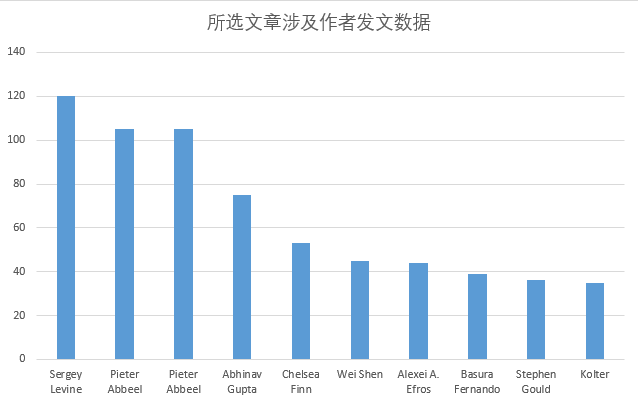
\includegraphics[width=.7\linewidth]{figure/fa.png}
    \caption{所选文章涉及作者发文数据图}
    \label{fig:fa}
\end{figure}

从\ref{table:a} 和 \ref{fig:fa} 中可以看出,发文数量最多的三位作者是Sergey Levine、Pieter Abbeel、Pieter Abbeel。但从\ref{table:a}
可以看出,虽然有些作者发文量不高,但是被引量很高。


\begin{table}[htbp]
    \centering
    \begin{tabular}{lc}
    \hline
    \textbf{国家} & \multicolumn{1}{l}{\textbf{数量}} \\ \hline
    美国          & 12                              \\
    英国          & 2                               \\
    法国          & 2                               \\
    中国          & 2                               \\
    以色列         & 1                               \\
    澳大利亚        & 1                               \\
    加拿大         & 1                               \\ \hline
    \end{tabular}
    \caption{所选文章涉及国家发文数据表}
    \label{table:b}
\end{table}

\begin{figure}[htbp]
    \centering
    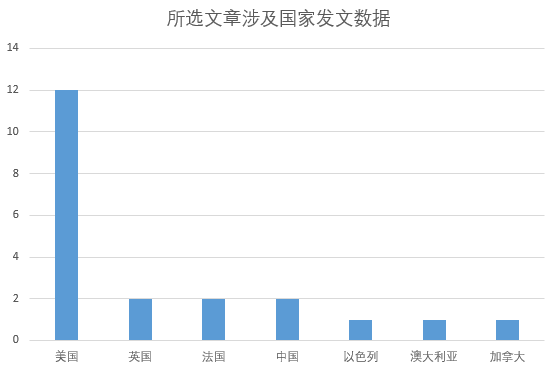
\includegraphics[width=.7\linewidth]{figure/fb.png}
    \caption{所选文章涉及国家发文数据图}
    \label{fig:fb}
\end{figure}

从\ref{table:b} 和 \ref{fig:fb} 可以看出,发文国家最多的是美国,呈现一超多强的格局。

\begin{table}[htbp]
    \centering
    \begin{tabular}{lc}
    \hline
    \textbf{机构}                          & \multicolumn{1}{l}{\textbf{数量}} \\ \hline
    Carnegie Mellon University           & 2                               \\
    University of Oxford                 & 2                               \\
    University of California,   Berkeley & 2                               \\
    Stanford University                  & 1                               \\
    Cornell University                   & 1                               \\
    Hebrew University                    & 1                               \\
    Rochester Institute of   Technology  & 1                               \\
    University of Michigan               & 1                               \\
    University of Washington             & 1                               \\
    google brain                         & 1                               \\
    University Paris-Est                 & 1                               \\
    The   Australian National University & 1                               \\
    Harvard University                   & 1                               \\
    Baidu Research                       & 1                               \\
    INRIA                                & 1                               \\
    Microsoft Research                   & 1                               \\
    Element AI                           & 1                               \\
    Johns Hopkins University             & 1                               \\
    Shanghai University                  & 1                               \\
    Cambridge                            & 1                               \\ \hline
    \end{tabular}
    \caption{所选文章涉及机构发文数据表}
    \label{table:c}
    \end{table}

    \begin{figure}[htbp]
        \centering
        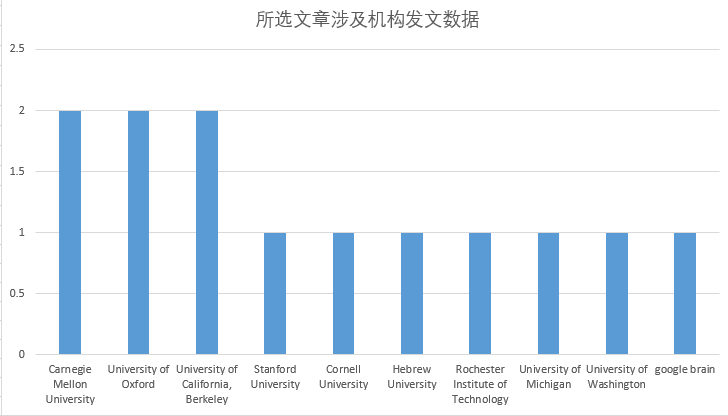
\includegraphics[width=.7\linewidth]{figure/fc.png}
        \caption{所选文章涉及机构发文数据图}
        \label{fig:fc}
    \end{figure}
    
    从\ref{table:c} 和 \ref{fig:fc} 可以看出,发文机构之间差距不大,大多机构是大学,大型科技企业。

    \begin{table}[htbp]
        \centering
        \begin{tabular}{lc}
        \hline
        \textbf{期刊会议}                                       & \textbf{次数} \\ \hline
        ICLR                                                & 6           \\
        PMLR                                                & 5           \\
        ICML                                                & 5           \\
        CVPR                                                & 5           \\
        NIPS                                                & 5           \\
        IEEE                                                & 4           \\
        Advances in neural information   processing systems & 3           \\
        arXiv                                               & 2           \\
        Journal of machine learning   research              & 1           \\
        Artificial intelligence review                      & 1           \\
        Learning to learn                                   & 1           \\
        ICCV                                                & 1           \\
        BMVC                                                & 1          
        \end{tabular}
        \label{table:d}
        \caption{所选文章涉及期刊发文数据表}
    \end{table}

    \begin{figure}[htbp]
        \centering
        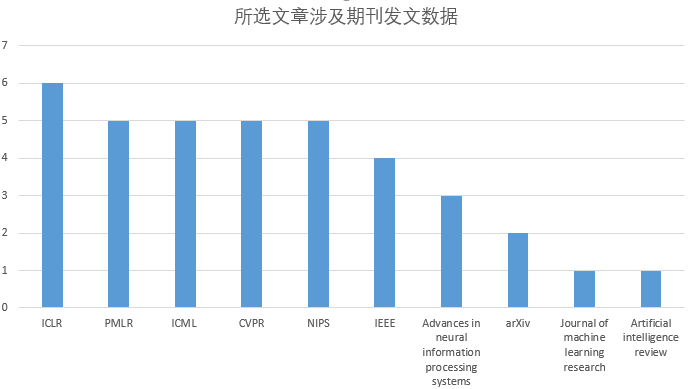
\includegraphics[width=.7\linewidth]{figure/fd.png}
        \caption{所选文章涉及机构发文数据图}
        \label{fig:fd}
    \end{figure}
    
    从\ref{table:d} 和 \ref{fig:fd} 可以看出,在元学习领域内,较为权威的期刊是 ICLR、PMLR、ICML、CVPR、NIPS。